En esta sección, vamos a comprobar empíricamente que nuestro algoritmo tiene una complejidad temporal de $O(n^2)$.

En este primer caso utilizamos instancias aleatorias variando el tamaño de entrada T(n). A su vez, utilizamos distintos tamaños de k. En la figura \ref{fig:problema2-k} se pueden observar los resultados obtenidos.

\begin{figure}[H]
  \begin{minipage}{0.5\linewidth}
    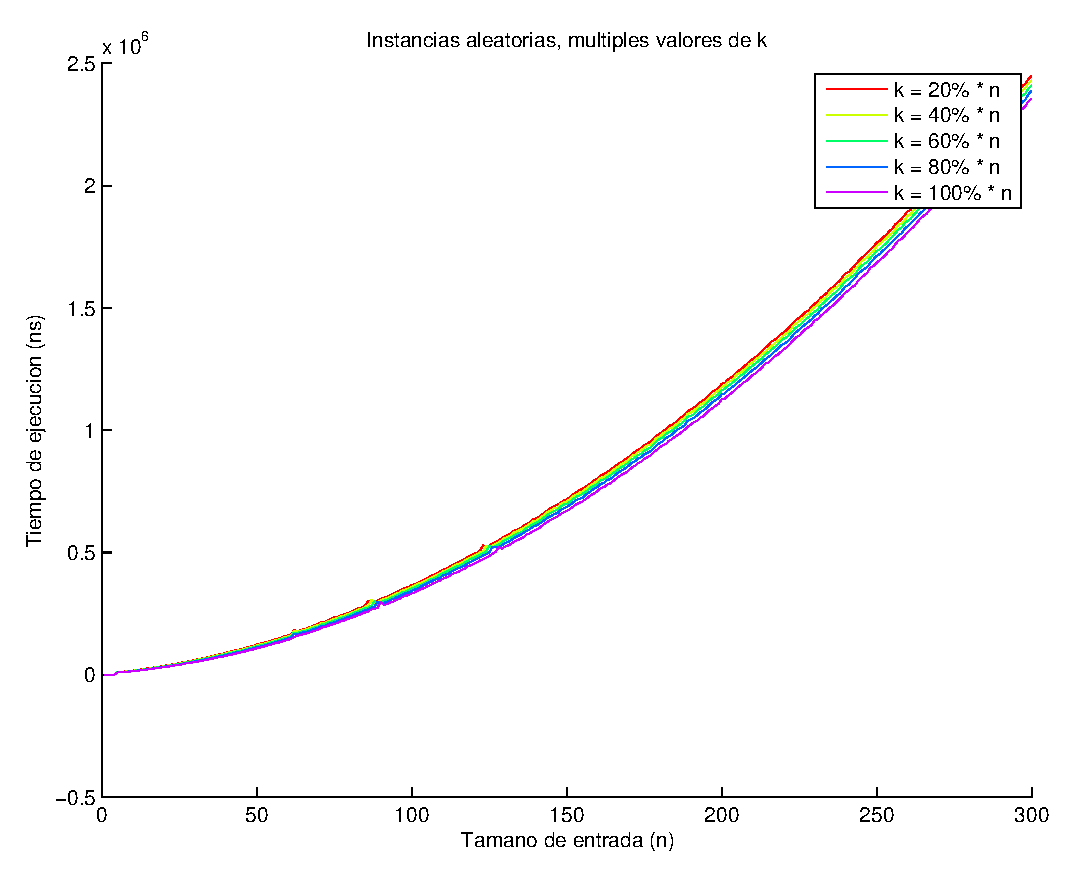
\includegraphics[width=\linewidth]{img/problema2/instancia_aleatoria_varios_k.eps}
\caption{Tiempo de ejecución instancia aleatoria}\label{fig:problema2-k}
\end{minipage}
  \hfill
  \begin{minipage}{0.5\linewidth}
    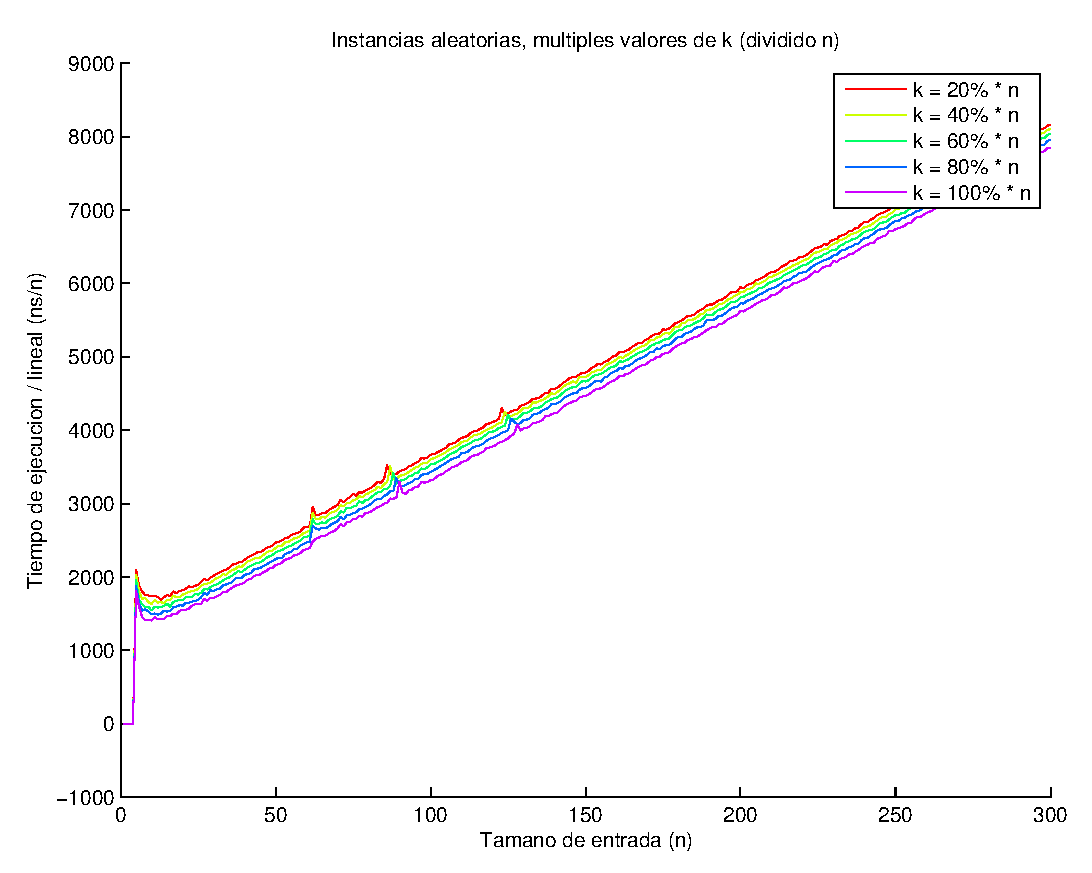
\includegraphics[width=\linewidth]{img/problema2/instancia_aleatoria_varios_k_div_n.eps}
    \caption{Idem, dividido por $n^2$}\label{fig:problema2-k-n}
  \end{minipage}	
\end{figure}

Además de presentar los datos como dijimos anteriormente en la figura \ref{fig:problema2-k}, incluimos otro gráfico donde mostramos donde se puede observar el comportamiento de T(n) cuando se lo divide por $n$. Hicimos esto porque en la figura \ref{fig:problema2-k} no hay nada que nos permita notar el comportamiento de $T(n)$ para los valores medidos.

Plasmamos los resultados de $T(n)/n$ en la figura \ref{fig:problema2-k-n}. En esta última figura, podemos observar claramente que $T(n) / n$ tiene un comportamiento lineal para los valores medidos, lo que nos dice que $T(n)$ tiene un comportamiento cuadrático para estos valores. De esta manera, pudimos comprobar empíricamente que $T(n)$ tiene una complejidad temporal de $O(n^2)$, lo cual demostramos anteriormente.